\documentclass[10pt]{beamer}
\usepackage[utf8]{inputenc}
\usepackage[vietnamese]{babel}
\usepackage{booktabs}
\usepackage{tabularx}
\usepackage{graphicx}
\IfFileExists{reports/figures/baseline-macro-metrics.png}{
    \graphicspath{{reports/figures/}}
}{
    \graphicspath{{figures/}}
}

\usetheme{Madrid}
\usecolortheme{default}
\setbeamercolor{block title alerted}{use=block title,fg=block title.fg,bg=block title.bg}
\setbeamercolor{block body alerted}{use=block body,fg=block body.fg,bg=block body.bg}
\setbeamertemplate{navigation symbols}{}

\title[Báo cáo tiến độ ĐATH]{BÁO CÁO TIẾN ĐỘ ĐỒ ÁN TỔNG HỢP}
\subtitle{Xây dựng hệ thống hỗ trợ chẩn đoán bệnh lý phổi từ ảnh X-quang lồng ngực sử dụng mô hình CNN/ViT và Grad-CAM}
\author[Bảo, Huy]{
    \textbf{Giảng viên hướng dẫn:}\\
    \vspace{0.1cm}
    PGS. TS. Quản Thành Thơ\\
    \vspace{0.5cm}
    \textbf{Thành viên tham gia:}\\
    \vspace{0.1cm}
    Quách Gia Bảo\\
    Dương Quốc Huy\\
}
\date{Báo cáo tiến độ ngày 26/10/2026}

\begin{document}

\begin{frame}
    \titlepage
\end{frame}

\begin{frame}{Công việc đã thực hiện}
    \begin{block}{Data Pipeline}
        \small
        \begin{itemize}
            \item Tiền xử lý 15.000 ảnh VinDr-CXR có ground truth.
            \item Chuẩn hóa kích thước ảnh và annotation.
            \item Hoàn thiện dataset, DataLoader và location masks.
        \end{itemize}
    \end{block}
    \vspace{0.2cm}
    \begin{block}{Classification Baselines}
        \small
        \begin{itemize}
            \item Huấn luyện ResNet-50, DenseNet-121, ViT-B/16.
            \item Hoàn thành artifact và đánh giá trên tập data test.
        \end{itemize}
    \end{block}
\end{frame}

\begin{frame}{Dữ liệu và annotation}
    \begin{block}{Tạo nhãn và location mask}
        \small
        \begin{itemize}
            \item 14 finding; Majority Vote dương khi ít nhất 2/3 bác sĩ đồng thuận.
            \item Soft-pixel Consensus hợp nhất bounding box theo mức đồng thuận từng pixel.
            \item Mask phục vụ localization và nghiên cứu location-aware loss.
        \end{itemize}
    \end{block}
    \vspace{0.15cm}
    \begin{block}{Chuẩn hóa ảnh}
        \small Resize về $224\times224$, chuyển thành 3 kênh để tương thích với pretrained ImageNet.
    \end{block}
\end{frame}

\begin{frame}{Chia tập dữ liệu}
    \begin{center}
        \small
        \begin{tabularx}{0.78\textwidth}{@{}Xrr@{}}
            \toprule
            \textbf{Tập} & \textbf{Ảnh} & \textbf{Tỷ lệ} \\
            \midrule
            Training & 10.500 & 70\% \\
            Validation & 2.250 & 15\% \\
            Internal Test & 2.250 & 15\% \\
            \textbf{Tổng} & \textbf{15.000} & \textbf{100\%} \\
            \bottomrule
        \end{tabularx}
    \end{center}
    \vspace{0.3cm}
    \begin{center}
        \begin{minipage}{0.88\textwidth}
            \begin{block}{Tổng kết}
                \small Nhóm đã hoàn thiện PyTorch Dataset và DataLoader, bảo đảm cả ba backbone sử dụng cùng dữ liệu, nhãn và quy trình tiền xử lý.
            \end{block}
        \end{minipage}
    \end{center}
\end{frame}

\begin{frame}{Training Framework và cấu hình}
    \begin{block}{Backbone}
        \small ResNet-50, DenseNet-121 và ViT-B/16 sử dụng pretrained ImageNet, với classification head gồm 14 logits.
    \end{block}
    \vspace{0.2cm}
    \begin{block}{Cấu hình huấn luyện}
        \small
        \begin{itemize}
            \item \textbf{Weighted Binary Cross-Entropy} để giảm ảnh hưởng của sự mất cân bằng lớp.
            \item Optimizer \textbf{AdamW} với learning rate \textbf{0.0001}, batch size \textbf{8} và tối đa \textbf{30 epochs}.
            \item Early stopping dựa trên \textbf{Macro-AUROC của tập validation}, với patience bằng \textbf{5}.
        \end{itemize}
    \end{block}
\end{frame}

\begin{frame}{Kết quả tổng quát trên Internal Test}
    \small
    \begin{tabularx}{\textwidth}{@{}Xrrr@{}}
        \toprule
        \textbf{Metric} & \textbf{ResNet-50} & \textbf{DenseNet-121} & \textbf{ViT-B/16} \\
        \midrule
        Macro-AUROC & 0.9401 & \textbf{0.9476} & 0.8458 \\
        Macro-AUPRC & 0.4470 & \textbf{0.4842} & 0.2015 \\
        Macro-Precision & \textbf{0.2532} & 0.2350 & 0.1185 \\
        Macro-Recall & 0.7831 & \textbf{0.8510} & 0.7250 \\
        Macro-F1 & \textbf{0.3564} & 0.3434 & 0.1881 \\
        \bottomrule
    \end{tabularx}

    \vspace{0.3cm}
    \begin{block}{Diễn giải}
        \small \textbf{DenseNet-121 đạt hiệu năng phân loại tốt nhất xét theo Macro-AUROC và Macro-AUPRC}, lần lượt là \textbf{0.9476} và \textbf{0.4842}. \\
        ResNet-50 có kết quả khá gần với DenseNet-121 và đạt \textbf{Macro-Precision} cùng \textbf{Macro-F1} cao hơn tại threshold \textbf{0.5}. \\
        Trong khi đó, \textbf{ViT-B/16} có hiệu năng thấp hơn đáng kể so với hai mô hình CNN trong cùng điều kiện thực nghiệm.
    \end{block}
\end{frame}

\begin{frame}{Macro Metrics: So sánh trực quan}
    \begin{center}
        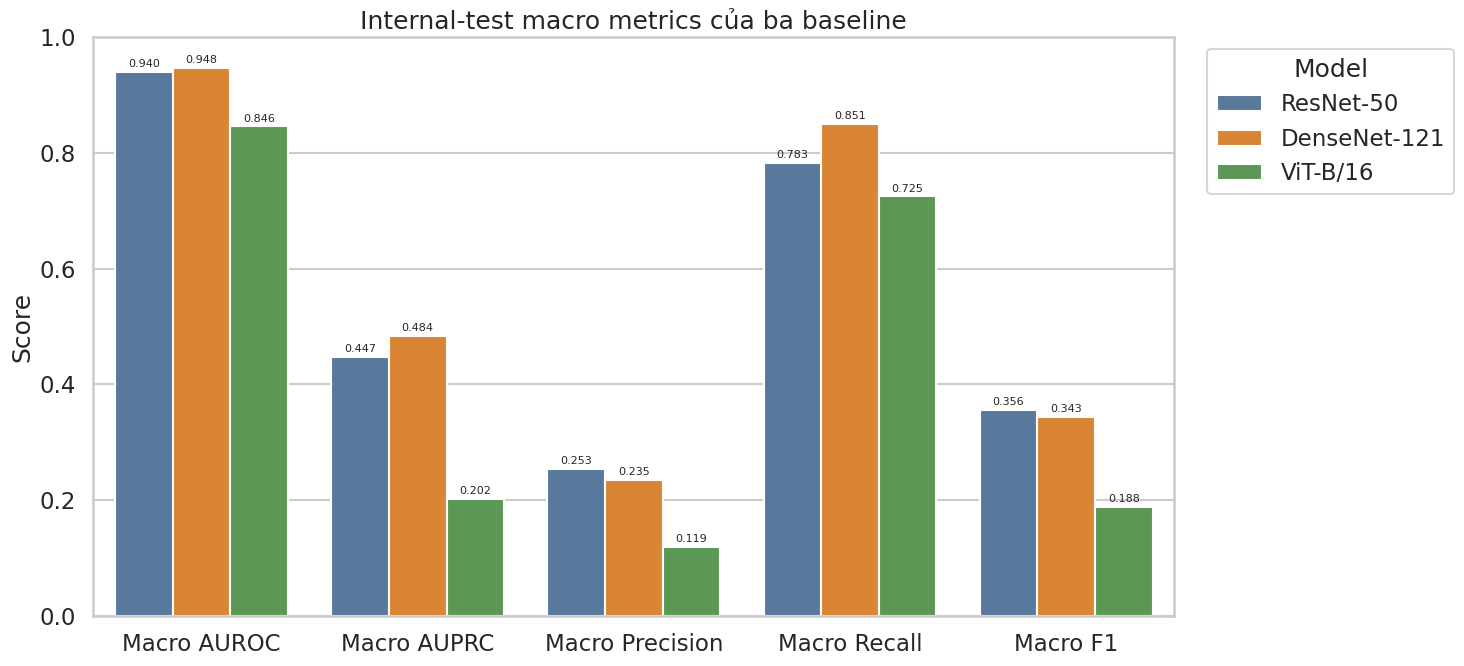
\includegraphics[width=0.9\textwidth,height=0.65\textheight,keepaspectratio]{baseline-macro-metrics.png}
    \end{center}
    \begin{alertblock}{Kết luận}
        DenseNet-121 dẫn đầu ở AUROC, AUPRC và Recall; ResNet-50 nhỉnh hơn ở Precision và F1. Cần cân nhắc nhiều metric thay vì chọn mô hình theo một điểm số duy nhất.
    \end{alertblock}
\end{frame}

\begin{frame}{Micro-average ROC và Precision--Recall}
    \begin{block}{Mất cân bằng và kết luận thực tiễn}
        \small
        \begin{itemize}\setlength{\itemsep}{0pt}
            \item Baseline PR khoảng 0.042, phản ánh tỷ lệ nhãn dương rất thấp.
            \item ResNet và DenseNet vượt ViT-B/16 trên cả hai đường cong.
            \item DenseNet-121 đạt Average Precision = 0.587, ResNet-50 đạt 0.573, trong khi ViT-B/16 chỉ đạt 0.296.
            \item Đường baseline của Precision–Recall nằm ở mức khoảng 0.042, phản ánh tỷ lệ nhãn dương thấp trong dữ liệu đánh giá.
        \end{itemize}
    \end{block}
    \begin{center}
        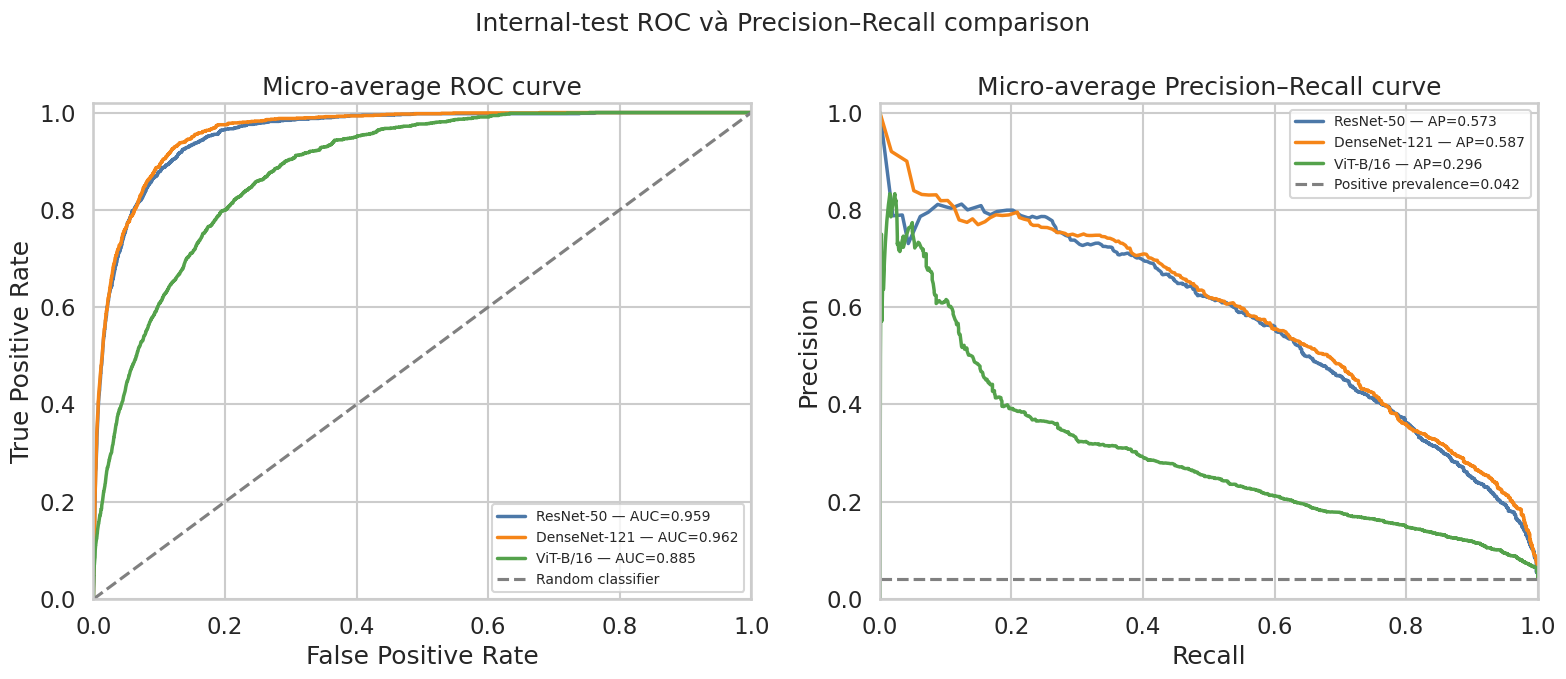
\includegraphics[width=0.96\textwidth,height=0.50\textheight,keepaspectratio]{roc-pr-curves.png}
    \end{center}
\end{frame}

\begin{frame}{Internal Test: Heatmap theo từng finding}
    \begin{center}
        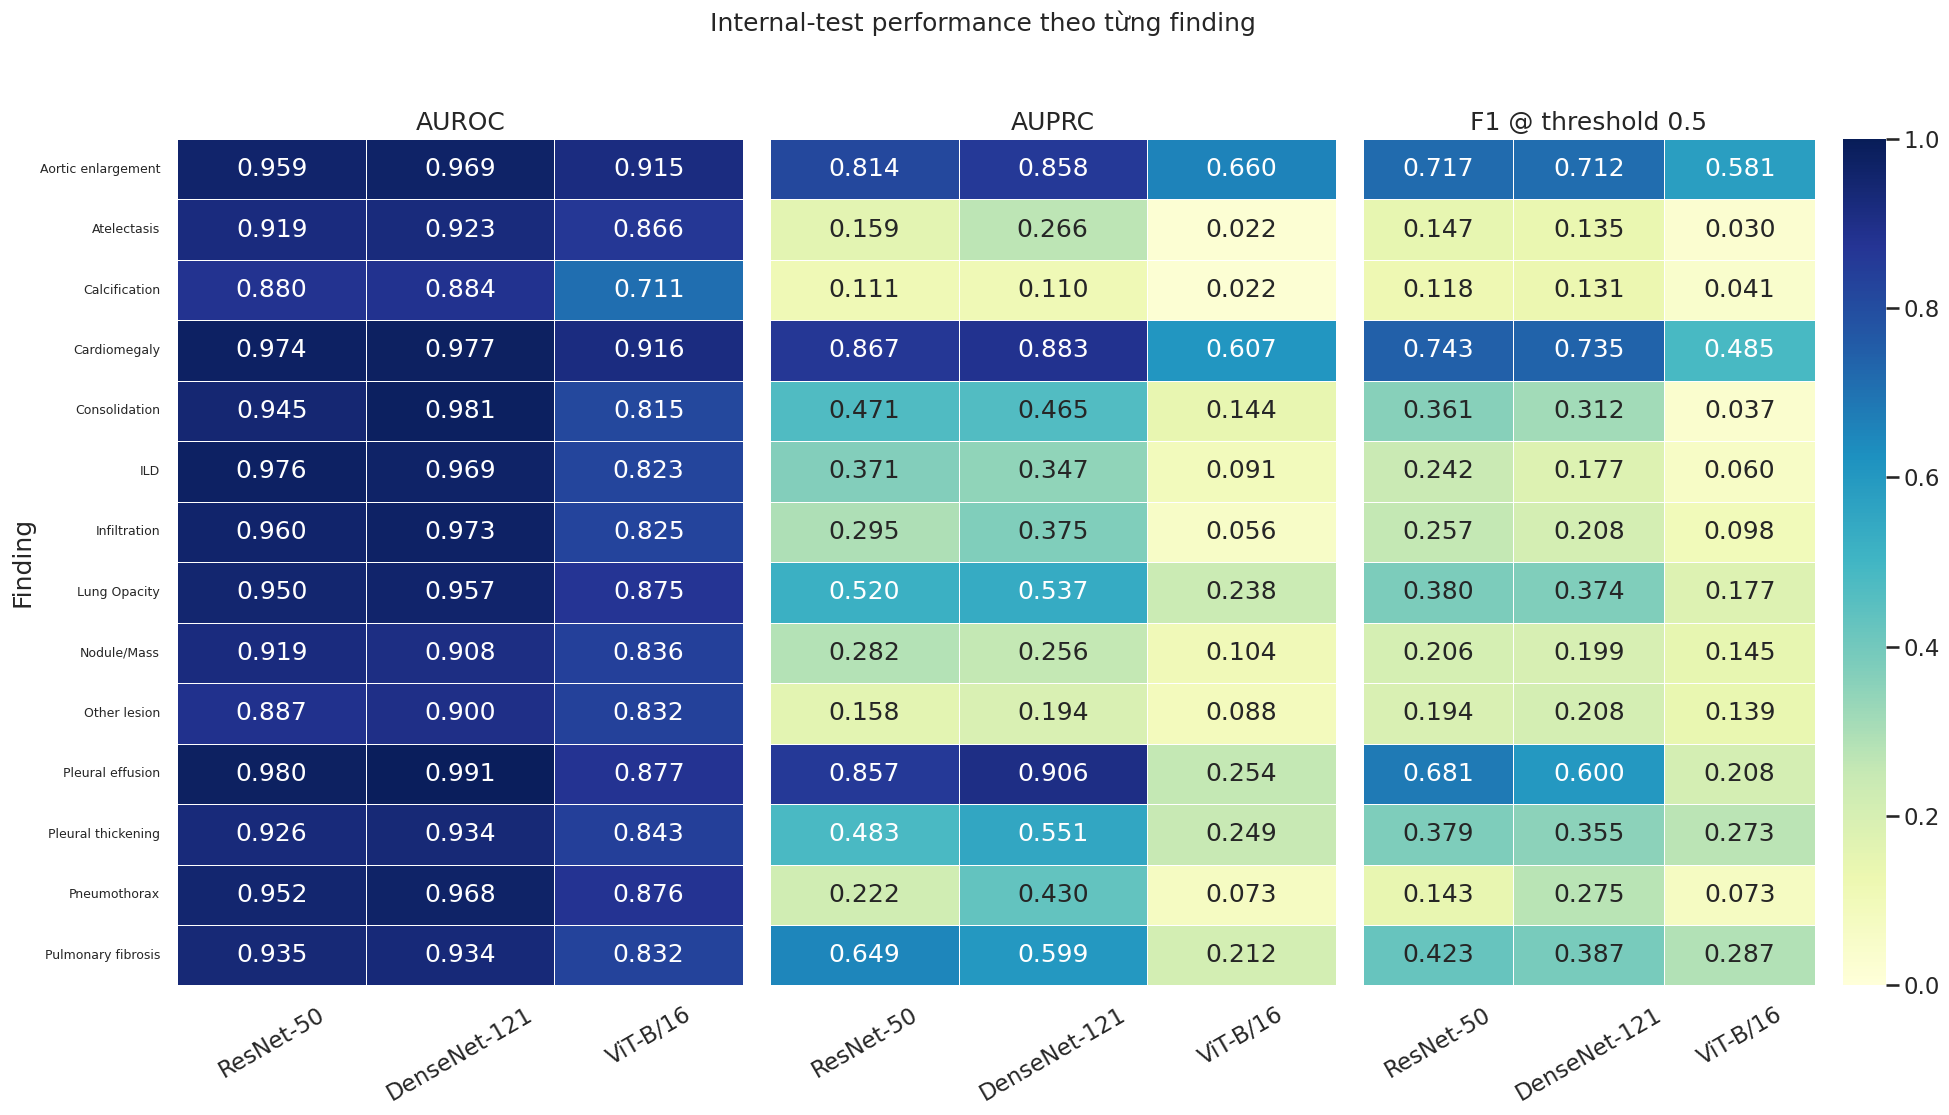
\includegraphics[width=0.96\textwidth,height=0.70\textheight,keepaspectratio]{per-finding-heatmap.png}
    \end{center}
    \scriptsize AUROC, AUPRC và F1 tại threshold 0.5 cho 14 finding trên ResNet-50, DenseNet-121 và ViT-B/16.
\end{frame}

\begin{frame}{Per-finding: nhóm phổ biến và nhóm khó}
    \begin{block}{Finding phổ biến}
        \small \textbf{Hiệu năng xuất sắc:} Hai mô hình CNN (DenseNet-121 \& ResNet-50) đạt kết quả rất cao trên các lớp tổn thương có tín hiệu thị giác rõ ràng (Cardiomegaly, Aortic enlargement, Pleural effusion).
    \end{block}
    \vspace{0.12cm}
    \begin{alertblock}{Lớp hiếm và khó phân biệt}
        \small Atelectasis và Pneumothorax có ít mẫu dương, tạo chênh lệch giữa khả năng xếp hạng và dự đoán thực tế. \\
        \vspace{0.1cm}
        \textbf{Atelectasis — DenseNet-121:}
        \begin{itemize}\setlength{\itemsep}{0pt}
            \item AUROC \textbf{0.923}: vẫn xếp hạng mẫu dương tốt.
            \item AUPRC \textbf{0.266} và F1 \textbf{0.135} tại threshold 0.5.
        \end{itemize}
    \end{alertblock}
\end{frame}

\begin{frame}{Insights từ Heatmap và hàm ý đánh giá}
    \begin{block}{So sánh kiến trúc}
        \small
        \begin{itemize}
            \item CNN vượt ViT-B/16 trên hầu hết các phát hiện dấu hiệu bất thường.
            \item Các bất thường trên ảnh phổ biến, có tín hiệu rõ thường tốt hơn phát hiện dấu hiệu bất thường hiếm hoặc mơ hồ.
            \item Ở lớp hiếm, AUROC cao nhưng AUPRC và F1 thấp xuất hiện phổ biến.
        \end{itemize}
    \end{block}
    \vspace{0.15cm}
    \begin{alertblock}{Nhận định và đánh giá}
        \small
        \begin{itemize}
            \item Mất cân bằng lớp là nguyên nhân cốt lõi làm giảm hiệu quả thực tế ở lớp hiếm.
            \item Cần phân tích riêng từng dấu hiệu bất thường, không chỉ dựa vào macro-average, để tránh đánh giá quá lạc quan.
        \end{itemize}
    \end{alertblock}
\end{frame}

\begin{frame}{Khó khăn hiện tại và hướng giải quyết}
    \small
    \renewcommand{\arraystretch}{1.2}
    \begin{tabularx}{\textwidth}{@{}p{0.3\textwidth}X@{}}
        \toprule
        \textbf{Khó khăn} & \textbf{Hướng giải quyết} \\
        \midrule
        \textbf{1. Mất cân bằng dữ liệu nghiêm trọng} & Tiếp tục sử dụng Weighted BCE; thử nghiệm Focal Loss hoặc Asymmetric Loss trong nghiên cứu mở rộng. Có thể áp dụng augmentation có kiểm soát cho lớp hiếm. \\
        \addlinespace[0.12cm]
        \textbf{2. Precision thấp dù Recall cao} & Tối ưu classification threshold theo từng lớp trên validation thay vì cố định 0.5. Phân tích False Positive để xác định các bất thường dễ bị dự đoán sai. \\
        \addlinespace[0.12cm]
        \textbf{3. AUROC cao nhưng AUPRC/F1 thấp} & Đánh giá đồng thời AUROC, AUPRC và F1 theo từng lớp; đối chiếu AUPRC với tỷ lệ positive của lớp. Phân tích riêng finding hiếm để tránh kết luận chỉ từ Macro-AUROC. \\
        \bottomrule
    \end{tabularx}
\end{frame}

\begin{frame}{Định hướng công việc tiếp theo}
    \begin{block}{Trả lời câu hỏi nghiên cứu RQ1}
        \small
        \textbf{RQ1:} \textit{Does better classification imply better localization?} Kiểm tra liệu mô hình phân loại tốt hơn có định vị vùng bất thường tốt hơn hay không.
        \begin{itemize}
            \item Triển khai Grad-CAM cho ResNet-50, DenseNet-121 và ViT-B/16; với ViT xử lý patch tokens thành biểu diễn không gian.
            \item Đánh giá bằng Pointing Game, Intersection over Union (IoU), Energy Inside Box (EIB).
            \item So sánh thứ hạng mô hình theo classification metrics với localization metrics để kiểm tra xem mô hình phân loại tốt hơn có thực sự định vị tốt hơn hay không
        \end{itemize}
    \end{block}
\end{frame}

\end{document}